\subsection{Возведение вполне упорядоченных множеств в степень: определение и свойства. Счётный ординал в счётной степени счётен.}

Возведение в целую положительную степень: ($\alpha ^ n$ есть произведение n сомножите-
лей, равных $\alpha$). Другими словами, если A упорядочено по типу $\alpha$, то множество $A^n$ последовательностей длины n с элементами из A с обратным лексикографическим порядком (сравнение справа налево) упорядочено по типу $\alpha^n$.

Следующий шаг — определить $\alpha^{\omega}$. Первая идея, приходящая в
голову — взять множество $A^{\mathbb{N}}$ бесконечных последовательностей и
определить на нём полный порядок. Но как его ввести — неясно. Поэтому можно попробовать определить возведение в степень индуктивно с помощью следующих соотношений:
$\alpha^0 = 1; \alpha^{\beta + 1} = \alpha^{\beta} \cdot \alpha; \alpha^{\gamma} = sup\{\alpha^{\beta} | \beta < \gamma \}$ для предельного $\gamma \neq 0$.

Теорема о трансфинитной рекурсии гарантирует, что эти соотношения однозначно определяют некоторую операцию над ординалами, которая и называется \textbf{возведением в степень}.

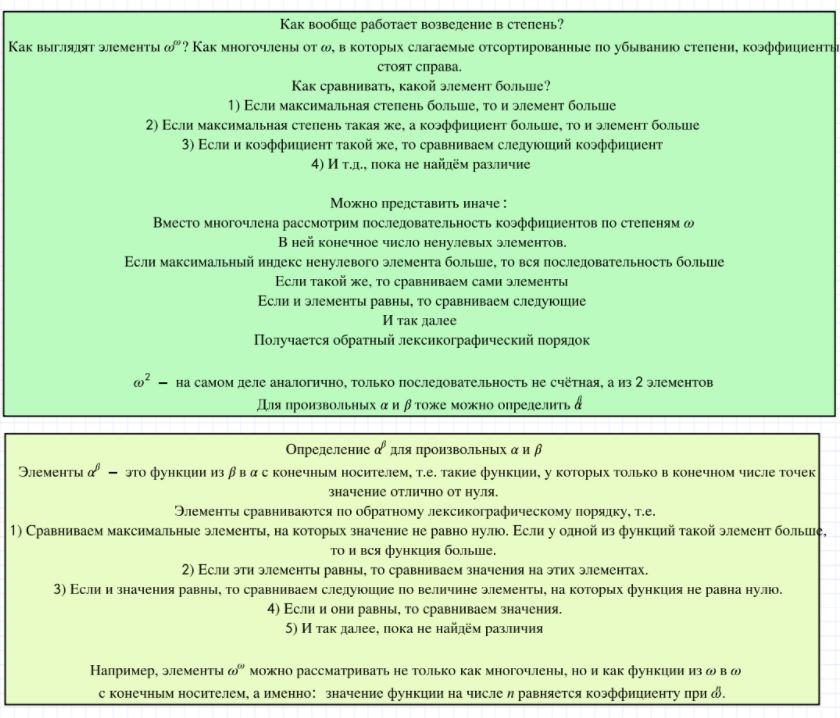
\includegraphics[]{images/2.4_degree}

\textbf{Свойства}:

1. $\alpha^{\beta + \gamma} = \alpha^{\beta} \cdot \alpha^{\gamma}$;

2. $(\alpha^{\beta})^{\gamma} = \alpha^{\beta \gamma}$

3. Если $\alpha > 1$, $\beta > 1$ то $\alpha^{\beta} > \alpha$.

$\blacktriangle$
1, 2: из индуктивного определения степени. Например, для 2: Для непредельного элемента - из определения, для предельного верно: $(\alpha^{\beta})^{\gamma} = sup\{(\alpha^{\beta})^{\xi} | \xi < \gamma \} = sup\{\alpha^{(\beta \xi)} | (\beta \xi) < \beta \gamma \} = \alpha^{\beta \gamma}$. Ура!

3:

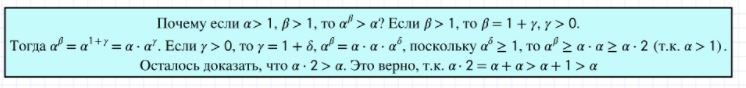
\includegraphics[]{images/2.4_degree2}
$\blacksquare$

\textbf{Теорема}. Если $\alpha$ и $\beta$ — счётные ординалы, то $\alpha^{\beta}$
счётный.

$\blacktriangle$
Если мы пронумеровали все элементы вполне упорядоченных множеств A и B, то любой элемент множества $[B \rightarrow A]$ может быть задан конечным списком натуральных чисел (носитель и значения
на элементах носителя), а таких списков счётное число.
$\blacksquare$